\documentclass[12pt]{article}
\usepackage[a4paper, text={6.5in,9in}]{geometry}
% \usepackage[utf8]{inputenc}
\usepackage{graphicx}
\graphicspath{ {immagini/} }

\usepackage{titling}

\usepackage{hyperref}
\hypersetup{
    colorlinks,
     citecolor=black,
     filecolor=black,
     linkcolor=black,
     urlcolor=black
 }

% \usepackage{fancyhdr}
% \pagestyle{fancy}

\usepackage{amsmath}
\usepackage{amssymb}
\usepackage{mathtools}
\usepackage{dsfont}
\usepackage{cases}
% \newcommand*{\Z}{\mathds{Z}}

\usepackage{minted, xcolor}
%\usemintedstyle{monokai}
\definecolor{bg}{HTML}{F0F0F0}
% \usepackage[defaultmono]{droidsansmono}
% \usepackage[T1]{fontenc}

\pretitle{%
  \begin{center}
  \LARGE
  \includegraphics[width=6cm]{logo-unipd} \\ [\bigskipamount]
}
\posttitle{\end{center}}

\title{\textbf{Università di Padova \\ Formal Methods for Cyber-Physical Systems project report}}
\author{Alberto Lazari - 2089120 \\ Elia Scandaletti - 2087934 \\ Francesco Protopapa - 2079466 \\}
\date{December 2022 - A.Y. 2022-2023}

\begin{document}
    \maketitle
    \pagebreak

    \tableofcontents
    \pagebreak

    \section{Notazione}
    \begin{description}
        \item $Post$: function which represents the set of states reachable from a given region by applying a single step of transition;
        \item $List[i]$: elemento di una lista $List$ di indice $Size(List) - i, i \in \mathbb N$.
    \end{description}

    \section{Reachability}
    \subsection{Intuitive idea}
    Given a region of initial states $Init$, a transition function $Trans$ and an invariant $Inv$, the goal of this algorithm is to decide if $Inv$ is verified in all the reachable states starting from $Init$ by applying $Trans$.

    To achieve this goal, a symbolic representation of all and only the reachable states of the system needs to be found. In this way, it is easy to check if the invariant is not verified in some of these states. An optimization can be used to avoid calculating all the states if some states that do not satisfy the invariant are found during the process.

    In order to do this, a variable $Reach$ is used to represent the reachable states of the system and it is updated iteratively.
    The basic idea is that at iteration $t$, $Reach$ represents all the states reachable from $Init$ by applying $Trans$ at most $t$ times.
    The algorithm stops when one of the following conditions is verified:
    \begin{enumerate}
        \item $Post(Reach) \subseteq Reach $: we have found all the reachable states;
        \item $Reach \cap NotInv \neq \emptyset$: we have found some reachable states in which the invariant is not verified.
    \end{enumerate}

    \textbf{TODO Disegnino}

    \subsection{Implementation}
    The implementation of the algorithm in pseudocode is the following:

    \begin{minted}[bgcolor=bg, breaklines, fontsize=\small, mathescape=true, escapeinside=||, linenos]{python}
function IsInvariantRespected(Init, Trans, Inv)
    NotInv |$\leftarrow \mathbb U\ \setminus$| Inv
    Reach |$\leftarrow$| Init
    New |$\leftarrow$| Init
    while New |$\neq \varnothing$| do
        if New |$\cap$| NotInv |$\neq \varnothing$| then
            return False
        end if
        New |$\leftarrow$| Post(New, Trans) |$\setminus$| Reach
        Reach |$\leftarrow$| Reach |$\cup$| New
    end while
    return True
end function
    \end{minted}

    For the Python implementation, it is sufficient to translate the following instructions:
    \begin{itemize}
        \item $A \leftarrow B$ becomes: \mintinline{python}{A = B}
        \item $\mathbb U\ \setminus A$ becomes: \mintinline{python}{~A}
        \item $A \neq \varnothing$ becomes: \mintinline{python}{not A.is_false()}
        \item $A \cap B \neq \varnothing$ becomes: \mintinline{python}{A.intersected(B)}
        \item $Post(A, Trans)$ becomes: \mintinline{python}{model.post(A)}
        \item $A \setminus B$ becomes: \mintinline{python}{A - B}
        \item $A \cup B$ becomes: \mintinline{python}{A + B}
    \end{itemize}

    \subsection{Proof of correctness}
    Let:
    \begin{itemize}
        \item $\mathbb U$ be the set of all the possible states of the model;
        \item $Inv \subseteq \mathbb U$ be the set of all the states that do satisfy the invariant;
        \item $NotInv \vcentcolon= \mathbb U \setminus Inv \subseteq \mathbb U$;
        \item $Reach^k$ be the set of all the states reachable in at most $k$ steps, defined as:
        $$
            \begin{cases}
                Reach^0 = Init \\
                Reach^{k + 1} = Reach^k \cup Post(Reach^k)
            \end{cases}
        $$
        \item $New^k$ be the set of all the states reachable in exactly $k$ steps, defined as:
        $$
            \begin{cases}
                New^0 = Init \\
                New^{k + 1} = Reach^{k+1} \setminus Reach^k
            \end{cases}
        $$
    \end{itemize}
    This way, $Reach^k$ and $New^k$ correspond to the values taken by the variables \texttt{Reach} and \texttt{New} at the $k$-th iteration.

    We want to prove that:
    \begin{itemize}
        % \item le definizioni date di $New^k$ e $Reach^k$ sono sound;
        \item the algorithm always terminates;
        \item $Reach^k \subseteq Inv\ \forall k$ se l'algoritmo ritorna true;
        \item if the algorithm returns true, then $Reach^k \subseteq Inv\ \forall k$;
        \item if the algorithm returns false, then $\exists k \mbox{ s.t. } Reach^k \cap NotInv \neq \varnothing$.
    \end{itemize}

    % \paragraph{Soundness of definitions}
    % \newcommand{\New}{\mathtt{New}}
    % \newcommand{\Reach}{\mathtt{Reach}}
    % Dimostriamo per induzione su $k$ che la definizione di $New$ e $Reach$ è corretta.
    % In particolare, dimostriamo che $New^k$ e $Reach^k$ corrispondono al valore delle variabili $\New^k$ e $\Reach^k$ al $k$-esimo ciclo dell'algoritmo.
    % Ovvero, vogliamo dimostrare che
    % \begin{equation}
    %     New^k = \New^k \wedge Reach^k = \Reach^k\ \forall k
    % \end{equation}

    % \subparagraph*{Caso base:}
    % $New^0 = Reach^0 = Init$ è corretto poiché corrisponde all'inizializzazione delle variabili nell'algoritmo.

    % \subparagraph*{Caso induttivo ($k+1$):}
    % Seguendo il flusso dell'algoritmo, assumendo che non sia già terminato, otteniamo:
    % \begin{equation}\label{th:sound:def_var}
    %     \begin{cases}
    %         \New^{k+1} = Post(\New^k) \setminus \Reach^k \\
    %         \Reach^{k+1} = \Reach^k \cup \New^k
    %     \end{cases}
    % \end{equation}

    % Inoltre, per definizione di $New$ e $Reach$ sappiamo che:
    % \begin{equation}\label{th:sound:def_ind}
    %     \begin{cases}
    %         Reach^{k+1} = Reach^k \cup Post(Reach^k) \\
    %         New^{k+1} = Reach^{k+1} \setminus Reach^k 
    %     \end{cases}
    % \end{equation}

    % Per ipotesi induttiva, sappiamo che:
    % \begin{equation*}
    %     \New^k = New^k \wedge \Reach^k = Reach^k
    % \end{equation*}

    % Sostituendo in (\ref{th:sound:def_var}), otteniamo
    % \begin{equation}\label{th:sound:def_var_sost}
    %     \begin{cases}
    %         \New^{k+1} = Post(New^k) \setminus Reach^k \\
    %         \Reach^{k+1} = Reach^k \cup New^k
    %     \end{cases}
    % \end{equation}

    % Per dimostrare che $\New^{k+1} = New^{k+1}\ \wedge\ \Reach^{k+1} = Reach^{k+1}$, per la (\ref{th:sound:def_ind}) e la (\ref{th:sound:def_var_sost}), è ora sufficiente dimostrare che
    % \begin{numcases}{}
    %     Reach^k \cup New^k = Reach^k \cup Post(Reach^k) \\
    %     Post(New^k) \setminus Reach^k = (Reach^k \cup New^k) \setminus Reach^k 
    % \end{numcases}

    \paragraph{Termination}
    We prove that the algorithm always terminates returning True or False.
    
    We know that $\mathbb U$ is finite, because every state is a combination of a finite and constant number of variables, which can assume a finite number of values.

    Furthermore, $\exists n$ such that:
    $$
    \begin{cases}
          New^k \subset New^{k+1} & \forall k < n \\
          New^k = New^{k+1} & \forall k \geq n
    \end{cases}
    $$

    Such $n$ must exist because the sequence $(Reach^k)_k$ is increasing (by definition of $Reach$), discrete (because it is a sequence of sets) and bounded above (because $Reach^k \subseteq \mathbb U\ \forall k$).

    As a consequence, by definition of $New$, $\exists n$ such that $New^{k+1} = \varnothing\ \forall k \geq n$.

    It follows that the algorithm exit the main loop after at most $n$ iterations and when it does, it returns True.

    \paragraph{Absense of false positives}

    We will prove that $Reach^k \subseteq Inv\ \forall k$ if the algorithm returns true.

    It is trivial to see that if the algorithm returns true, then the while loop terminates after $k$ iterations because $New^k = \varnothing$ and in every previous iteration we did not enter the condition on line 6 ($New^{k'} \cap NotInv = \varnothing\ \forall k' < k$).
    Furthermore, $New^k = \varnothing \subseteq Inv$.

    Therefore, it is possible to say that if the algorithm returns true then $New^{k'} \subseteq Inv\ \forall k' \leq k$.

    By induction on $k$ we prove that
    \begin{equation}\label{th:true:tesi}
        New^{k'} \subseteq Inv\ \forall k' \leq k \implies Reach^k \subseteq Inv
    \end{equation}
    
    \subparagraph*{Base case:}

    if $k = 0$ then $Reach^0 = Init = New^0$ by definition of $Reach$ and $New$. Therefore, $New^0 \subseteq Inv \implies Reach^0 \subseteq Inv$ is trivially true.

    \subparagraph*{Inductive case ($k+1$):}

    We want to inductively prove that:
    \begin{equation}\label{th:true:ind:tesi}
        New^{k'} \subseteq Inv\ \forall k' \leq k+1 \implies Reach^{k+1} \subseteq Inv
    \end{equation}
    We can assume that $New^{k'} \subseteq Inv\ \forall k' \leq k+1$, otherwise the left part of (\ref{th:true:ind:tesi}) is false and, therefore, the inductive case is trivially true.

    So we want to prove $Reach^{k+1} \subseteq Inv$ assuming that:
    \begin{numcases}{}
        New^{k'} \subseteq Inv\ \forall k' \leq k+1 & \mbox{as just said} \label{th:true:ind:ass_1} \\
        New^{k'} \subseteq Inv\ \forall k' \leq k \implies Reach^k \subseteq Inv & \mbox{by inductive hypothesis} \label{th:true:ind:hp_ind} \\
        Reach^{k+1} = Reach^{k} \cup New^{k+1} & \mbox{by definition of $New$} \label{th:true:ind:def_new}
    \end{numcases}

    It is trivial to see that from (\ref{th:true:ind:ass_1}) follows
    \begin{numcases}{}
        New^{k'} \subseteq Inv\ \forall k' \leq k \label{th:true:ind:hp_ind:left} \\
        New^{k+1} \subseteq Inv \label{th:true:ind:new}
    \end{numcases}

    (\ref{th:true:ind:hp_ind}) and (\ref{th:true:ind:hp_ind:left}) imply that
    \begin{equation}\label{th:true:ind:hp_ind:right}
        Reach^k \subseteq Inv
    \end{equation}

    Finally, from (\ref{th:true:ind:def_new}), (\ref{th:true:ind:new}) and (\ref{th:true:ind:hp_ind:right}) follows the inductive thesis (\ref{th:true:ind:tesi}).

    
    \paragraph{Absense of false negatives}
    We prove that if the algorithm returns false, then $\exists k \mbox{ s.t. } Reach^k \cap NotInv \neq \varnothing$.

    It is trivial to see that the only case in which the algorithm returns false is when at iteration $k$ the condition $New^k \cap NotInv \neq \varnothing$ is verified.
    
    \section{Counterexample search}
    \subsection{Intuitive idea}
    On every iteration of the reachable states search, the $New$ set is stored in a list.
    If $New \cap NotInv = \varnothing$ for a specific iteration, $New \cap NotInv$ is added to the list, that is the set of states in which the invariant is not satisfied, instead of $New$.
    The trace of states that leads the system not to satisy the invariant is recursively built using the list, following this procedure:
    \begin{itemize}
        \item \textbf{Base case:} If the list only contains an element E, return one out of any the states in E;
        \item \textbf{Recursive case:} Otherwise:
        \begin{enumerate}
            \item pick the last element \texttt{sym\_target} and remove it from the list;
            \item choose \texttt{target} out of any of the states in \texttt{sym\_target};
            \item reduce the states in the last element of the list in a way such that \texttt{target} is reachable from each state in it in a single iteration;
            \item recursively invoke the procedure with on the modified list and concatenate the result with \texttt{target}.
        \end{enumerate}
    \end{itemize}
    This algorithm allows to always choose one out of any element in the region placed in the list tail.
    The procedure step in which the last element of the list is modified before the recursive step is needed in order to keep this property valid.

    \begin{figure}[H] 
        \centering
        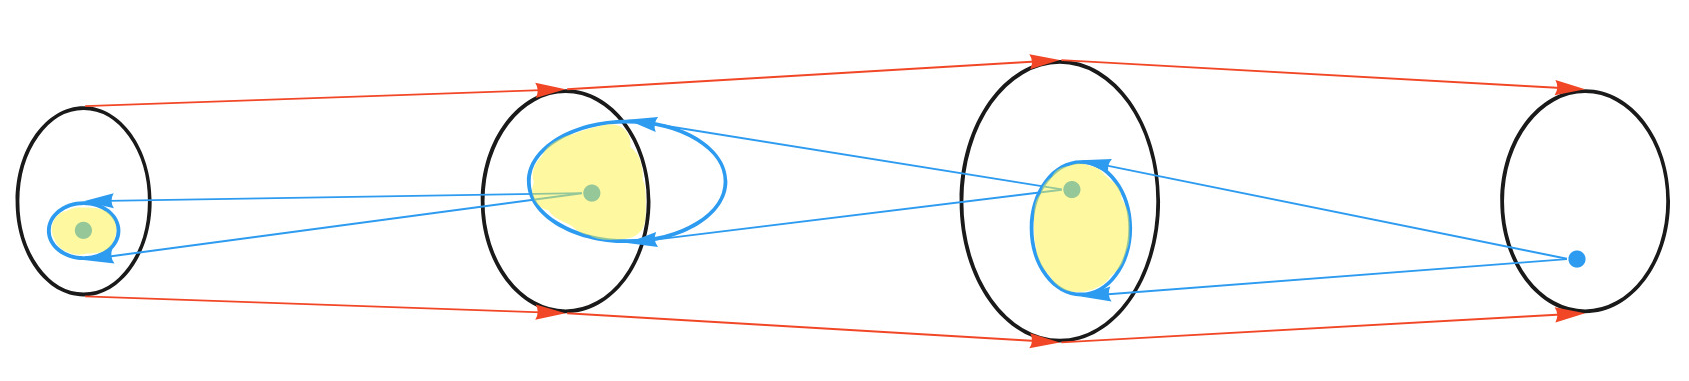
\includegraphics[width=\textwidth]{backtrace-diagram.png}
        \caption{Diagram representing the backtrace creation process.}
    \end{figure}

    \subsection{Implementation}
    Here is the pseudocode for the trace creation algorithm:
    \begin{minted}[bgcolor=bg, breaklines, fontsize=\small, mathescape=true, escapeinside=||, linenos]{python}
function CreateTrace(SymTrace)
    if len(SymTrace) == 0 return []
    if len(SymTrace) == 1 return [PickOneState(SymTrace[0])]

    SymTarget |$\leftarrow$| SymTrace.pop()
    Target |$\leftarrow$| PickOneState(SymTarget)
    SymTrace[-1] = SymTrace[-1] |$\cap$| Pre(Target)
    Trace |$\leftarrow$| CreateTrace(SymTrace)
    Trace |$\leftarrow$| Trace + Target
    return Trace
end function
    \end{minted}
    Let $Trace$ be the state list obtained from the \mintinline{python}{CreateTrace(SymTrace)} function. To get the inputs that lead the system from a state in $Trace$ to its successor, it is possible to apply the function \mintinline{python}{GetInputsBetweenStates(State1, State2)} on two adjacent states in the list.
    
    \subsection{Proof of correctness}
    \begin{itemize}
        \item Precondition:
        \begin{equation}
            \begin{cases}
                i \neq j \implies SymTrace[i] \cap SymTrace[j] = \varnothing\ \forall i, j \\
                SymTrace[i] = R \wedge \exists SymTrace[i+1] \implies SymTrace[i+1] \subseteq Post(R)
            \end{cases}
        \end{equation}
        \item Postcondition: The function returns a list of states (Trace) that satisfies the following conditions:
        \begin{equation}
            \begin{cases}
                SymTrace[i] = R \implies Trace[i] \in R \\
                \forall i \mbox{ s.t. } 0 \leq i < SymTrace.size - 1, Trace[i+1] \in Post(\{Trace[i]\})
            \end{cases}
        \end{equation}
    \end{itemize}

    \subparagraph*{Base case - SymTrace is empty}
    We return an empty list that trivially satisfies both postconditions.

    \subparagraph*{Base case - SymTrace has only one element}

    SymTrace is made of a single region R and we return a list made of one state in R.
    SymTrace[0] = R and Trace[0] $\in$ R.
    The second postcondition is trivially true because Trace has only one element.

    \subparagraph*{Recursive case}
    SymTrace has at least two elements.
    
    SymTrace' is the original value of SymTrace.

    \begin{minted}[bgcolor=bg, breaklines, fontsize=\small, mathescape=true, escapeinside=||]{python}
SymTarget |$\leftarrow$| SymTrace.pop()
Target |$\leftarrow$| PickOneState(SymTarget)
    \end{minted}

    Target $\in$ SymTrace[-1] because of the properties of the PickOneState function.

    SymTrace is equal to SymTrace' without its last element.
     
    \begin{minted}[bgcolor=bg, breaklines, fontsize=\small, mathescape=true, escapeinside=||]{python}
    SymTrace[-1] = SymTrace[-1] |$\cap$| Pre(Target)
    \end{minted}

    Target $\in$ Post(\{s\}) $\forall$ s $\in$ SymTrace[-1]

    The precondition of the recursive call is satisfied because:
    \begin{itemize}
        \item if SymTrace' is a list of disjoint regions then SymTrace[0:-1] = SymTrace'[0:-2] is a list of disjoint regions;
        moreover, SymTrace[-1] $\subseteq$ SymTrace'[-2] implies that SymTrace[-1] is disjoint from all the other elements of SymTrace;
        \item By the precondition and that $\forall i \mbox{ t.c. } 0 \leq i < SymTrace.size - 1 : SymTrace[i] = Symtrace'[i]\ e\ SymTrace[-1] \subseteq SymTrace'[-2] $, then
        \begin{equation}
            \forall i \mbox{ s.t. } 1 \leq i < SymTrace.size, \forall e \in SymTrace[i],  e \in Post(SymTrace[i-1])
        \end{equation}
    \end{itemize}

    \begin{minted}[bgcolor=bg, breaklines, fontsize=\small, mathescape=true, escapeinside=||]{python}
 Trace |$\leftarrow$| CreateTrace(SymTrace)
    \end{minted}

    so Trace' = CreateTrace(SymTrace) respects the postcondition of CreateTrace.
    
    \begin{minted}[bgcolor=bg, breaklines, fontsize=\small, mathescape=true, escapeinside=||]{python}
    Trace |$\leftarrow$| Trace + Target
    \end{minted}

    The postcondition is satisfied if:
    \begin{numcases}{}
        SymTrace[i] = R \implies Trace[i] \in R; \label{th:trace:ric:dim-post:1} \\
        \forall i \mbox{ s.t. } 0 \leq i < SymTrace.size - 1, Trace[i+1] \in Post(\{Trace[i]\}). \label{th:trace:ric:dim-post:2}
    \end{numcases}

    (\ref{th:trace:ric:dim-post:1}) is satisfied:
    \begin{itemize}
        \item for all the elements of Trace except the last one, because of the postcondition of the recursive call;
        \item for the last element of Trace = Target $\in$ SymTrace[-1], because obtained by PickOneState(SymTrace[-1]).
    \end{itemize}

    (\ref{th:trace:ric:dim-post:1}) is satisfied:
    \begin{itemize}
        \item $\forall i \mbox{ s.t. } 0 \leq i < SymTrace.size - 2$ following the recursive call postcondition;
        \item Trace[-1] = target $\in Post(\{Trace[-2]\})$, because target is obtained by PickOneState(SymTrace[-1]) and SymTrace[-1] $\subseteq$ Post(SymTrace[-2]).
    \end{itemize}
\end{document}
